\documentclass[a4paper, 12pt, titlepage, oneside]{article}

\usepackage[francais]{babel}
\usepackage{fancyhdr}
\usepackage{graphicx}
\usepackage{amsmath}
\usepackage{subcaption}

\graphicspath{ {images/}}

\author{Martin Olivier, Fabien Goglio}
\title{Rapport InSite}

\pagestyle{fancy}

%Put the chapter and section header in lowercase
%\renewcommand{\chaptername}[1]{%
%	\markboth{#1}{}}

\renewcommand{\sectionmark}[1]{%
	\markright{\thesection\ #1}}

%delete the current header
\fancyhf{}

\fancyhead[LE, RO]{\bfseries\thepage}
\fancyhead[LO]{\bfseries\textit\rightmark}
%\fancyhead[RE]{\bfseries\textit}
\fancyhead[RE]{WAT}
\renewcommand{\footrulewidth}{0.5pt} %space for the rule
\fancypagestyle{plain}{\fancyhead{}, %get rid of header on plain pages
	\renewcommand{\headrulewidth}{0pt} % and the line
}


\begin{document}
\maketitle

\pagenumbering{roman}
\newpage
	\tableofcontents
\newpage
\cleardoublepage
\pagenumbering{arabic}
\section{Remerciement}
	Nous tenons a remercier \[...\]
	\newpage
\section{Introduction}
	\newpage
\section{Presentation}
	\subsection{Description}
		InSite analyse et detecte des objets archeologiques dans des releves geomagnetiques, en utilisant des techniques novatrices dans le domaine de
		la Computer Vision, ainsi que de l'apprentissage automatique.
	\subsection{Objectifs}
	Nous cherchons a:
	\begin{itemize}
		\item Manger 
		\item Boire
	\end{itemize}

	\newpage

\section{Cadrage}
	\subsection{Budget}
	\subsection{Dates clefs}
	\subsection{Organisation}
	\subsubsection{Demarche}
	\subsection{Planning}
	\newpage
\section{Demarche Initiale}
	\subsection{Detections de formes}

	\subsubsection{Filtrage}
	{TODO: REMPLIR}
	
	\subsubsection{Algorithmes de detections de bords}
	Nous avons debuter nos recherches avec une solution evidente, l'Algorithme de Canny. Cet algorithme fonctionne en plusieurs etapes:
	\begin{enumerate}
		\item \textbf{Reduction du bruit:}\\
			\indent On applique un filtre Gaussien 5x5 pour reduire le bruit present dans l'image
		\item \textbf{Recherche du gradient d'intensite de l'image:}\\  
		 	\indent On applique ensuite un kernel de Sobel sur l'image "lisse" dans les directions verticales et horizontales afin d'obtenir les derives premieres dans
		la direction verticale $G_x$ et horizontales $G_y$. Le gradient de bord est donne par l'equation
			\begin{align}
				\nabla (G) & = \sqrt{G_x^2 + G_y^2}\\
				Angle (\theta) & = \tan^{-1}(\frac{G_x}{G_y})
			\end{align}
		Le gradient est toujours orthogonal au bord.

		\item \textbf{Suppression des non maximums locaux}\\
			\indent Une fois les gradients obtenus, on analyse tout les pixels de l'image, et on determine si le pixel est un maximum local dans la
			direction du gradient. \\
			Si oui, c'est un bord et sa valeur est garde pour la prochaine etape, sinon, elle est mise a 0. On obtient une image binaire, avec que des bords

		\item \textbf{Seuil d'Hysterisis} \\
			\indent On utilise deux seuils, $minVal$ et $maxVal$. Tout les bords ayant une intensite de gradient superieur a $maxVal$ est forcement un
			bord, ceux en dessous de $minVal$ sont forcement des non-bords, et sont donc abandonne. Les bords qui sont entre ces deux seuil sont classe
			"bords" ou "non-bords" selon leur connectivite. Si ils sont connecte a des pixels qui sont des forcement des bords, alors ce sont des bords,
			sinon, ils sont aussi abandonne.\\
		
	\end{enumerate}
	\newpage
	On obtient ce genre d'image:\\
	\begin{figure}[!h]
		\centering
		\begin{subfigure}[b]{0.4\linewidth}
			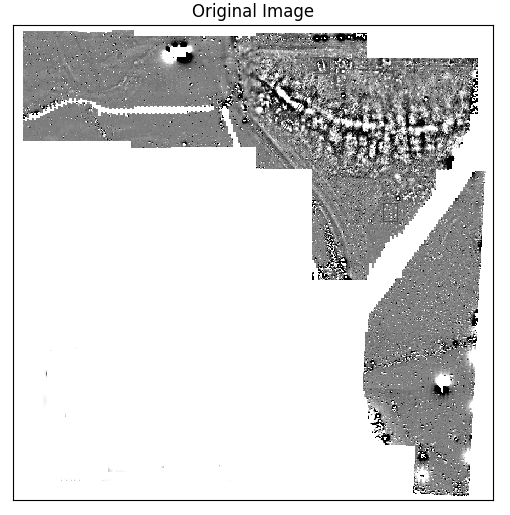
\includegraphics[width=\linewidth]{Canny1a.png}
			\caption{Image originelle}
		\end{subfigure}
		\begin{subfigure}[b]{0.4\linewidth}
			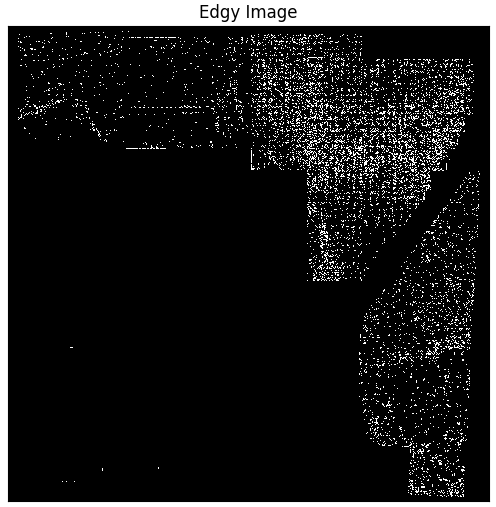
\includegraphics[width=\linewidth]{Canny1b.png}
			\caption{Image traite avec Canny}
		\end{subfigure}
		\label{fig:canny}
	\end{figure}
	
	On observe que l'algorithme ne parvient a trouver les contours des objets d'interet. Cela est du a la haute quantite de bruit que l'on trouve dans l'image. On 
	peut cependant trouver une densite de points plus eleve aux endroits d'interets.
	TODO: AJOUTER PHOTO DETAILS 
	Malgres des resultats peu encouragant avec des algorithmes classiques, nous avons decide d'utiliser un autre algorithme, celui
	
	\subsubsection{Problemes rencontres}
	TODO: A REMPLIR
	
\newpage
\section{Developement d'une nouvelle methodologie}
	\subsection{Detections de bruits par reseaux neuronal}
	\subsubsection{Caracterisation}
	\subsubsection{Explication de l'approche}
	\subsubsection{Problemes initiaux}
	\subsubsection{Solutions}
	\subsubsubsection{Generation d'exemple}
	Classifier a la main tout les exemples necessaires a l'entrainement du reseau etait une tache surhumaine. Par soucis d'efficacite, nous avons decide de construire nous meme
	nos exemples, et des les utiliser en combination avec des exemples provenant des images, et classifie a la main.
	Pour avoir une meilleure chance de creer un bruit proche de la realite, nous avons utilise 2 approches differentes:
	\begin{itemize}
		\item Une approche informatique
		\item Une approche mathemathique
	\end{itemize}
	L'approche informatique consiste a creer 2 cercles, de tailles variables,un noir et un blanc, ayant la meme origine. Ces cercles sont imprime sur une \quote{backplate} grise
	avec du bruit genere aleatoirement. Afin d'ameliorer le resultat, du bruit est ajoute aux cercles, augmentant particulierement aux bords de ceux ci.
		
	Nous avons genere une fonction mathematique se rapprochant de celle d'un dipole. 
	\subsubsubsection{Traitement des images}
	TODO : Parler de la preparation du dataset (decoupage, ajout de bruit sur nos exemples reel etc)
	TODO : Expliquer le fait qu'on a pas eu le temps d'implementer
\newpage
\section{Bilan provisoire et perspectives}
	\subsection{Bilan} %Changer le nom ?
	\subsection{Implementation d'un reseau convolutionnel}
	\subsection{Choix de la direction de recherche}

\newpage
\section{Annexes}

\end{document}
